\documentclass[pdflatex,compress,mathserif]{beamer}

%\usetheme[dark,framenumber,totalframenumber]{ElektroITK}
\usetheme[darktitle,framenumber,totalframenumber]{ElektroITK}

\usepackage[utf8]{inputenc}
\usepackage[T1]{fontenc}
\usepackage{lmodern}
\usepackage[bahasai]{babel}
\usepackage{amsmath}
\usepackage{amsfonts}
\usepackage{amssymb}
\usepackage{graphicx}
\usepackage{multicol}
\usepackage{lipsum}
\usefonttheme[onlymath]{serif}

\newcommand*{\Scale}[2][4]{\scalebox{#1}{$#2$}}%

\setbeamertemplate{caption}[numbered]

\title{MATEMATIKA DASAR}
\subtitle{Pembahasan Soal Pretest}

\author{Mifta Nur Farid}

\begin{document}
	
	\maketitle
	
	\section{Pembahasan Soal Pretest}

	\begin{frame}
		\frametitle{Pembahasan Soal Pretest}
		\begin{center}
			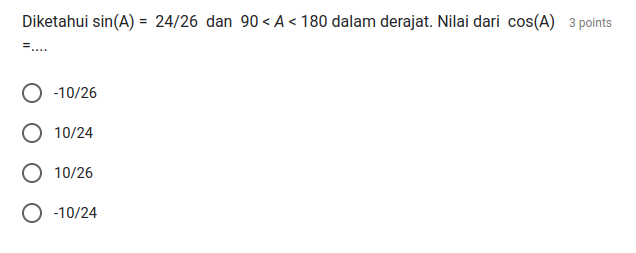
\includegraphics[width=\linewidth]{img/img01}
		\end{center}
	\end{frame}
	
	\begin{frame}
		\frametitle{Pembahasan Soal Pretest}
		\begin{center}
			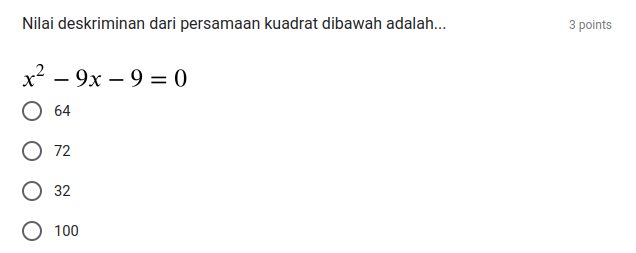
\includegraphics[width=\linewidth]{img/img02}
		\end{center}
	\end{frame}
	
	\begin{frame}
		\frametitle{Pembahasan Soal Pretest}
		\begin{center}
			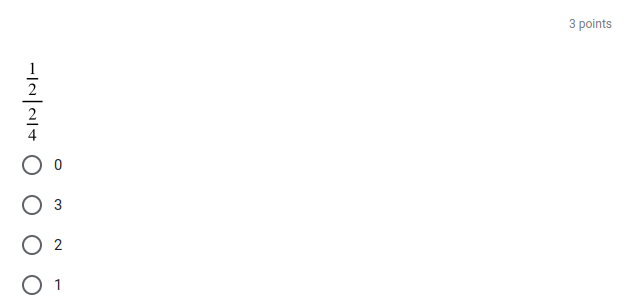
\includegraphics[width=\linewidth]{img/img03}
		\end{center}
	\end{frame}
	
	\begin{frame}
		\frametitle{Pembahasan Soal Pretest}
		\begin{center}
			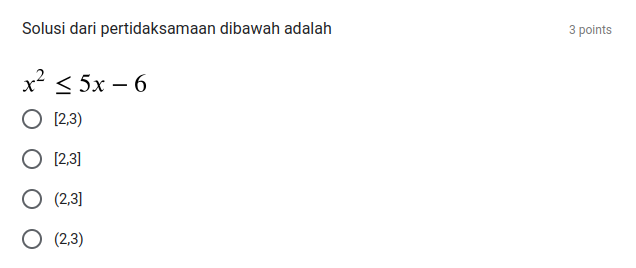
\includegraphics[width=\linewidth]{img/img04}
		\end{center}
	\end{frame}
	
	\begin{frame}
		\frametitle{Pembahasan Soal Pretest}
		\begin{center}
			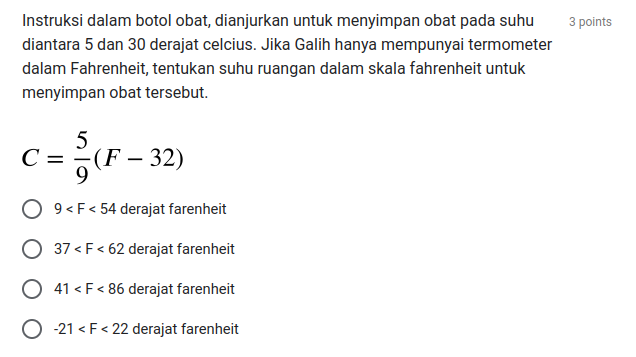
\includegraphics[width=\linewidth]{img/img05}
		\end{center}
	\end{frame}
	
	\begin{frame}
		\frametitle{Pembahasan Soal Pretest}
		\begin{center}
			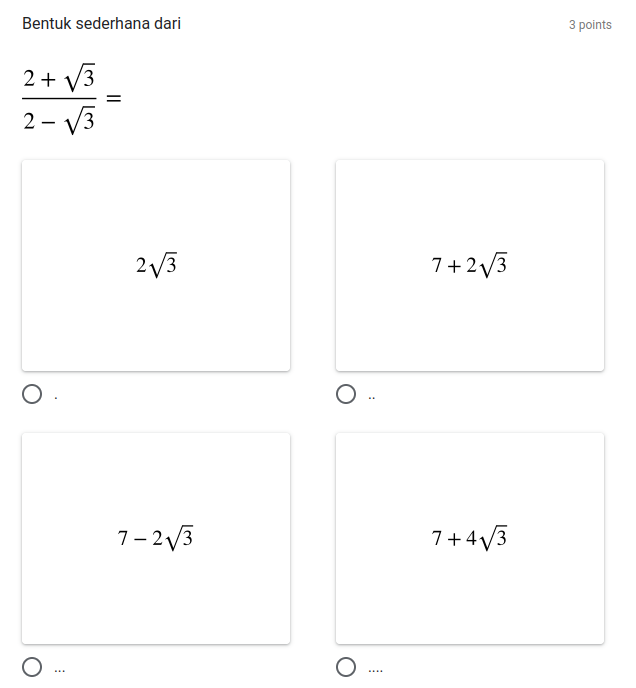
\includegraphics[width=0.6\linewidth]{img/img06}
		\end{center}
	\end{frame}
	
	\begin{frame}
		\frametitle{Pembahasan Soal Pretest}
		\begin{center}
			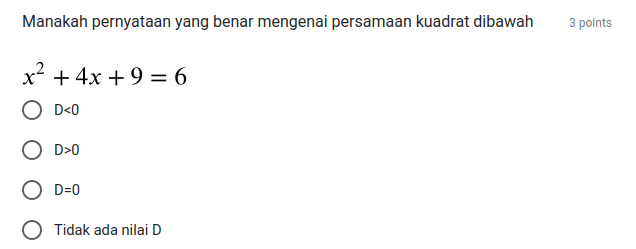
\includegraphics[width=\linewidth]{img/img07}
		\end{center}
	\end{frame}
	
	\begin{frame}
		\frametitle{Pembahasan Soal Pretest}
		\begin{center}
			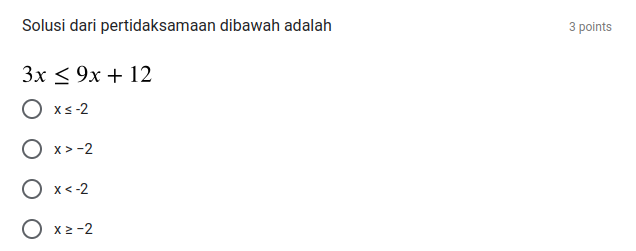
\includegraphics[width=\linewidth]{img/img08}
		\end{center}
	\end{frame}
	
	\begin{frame}
		\frametitle{Pembahasan Soal Pretest}
		\begin{center}
			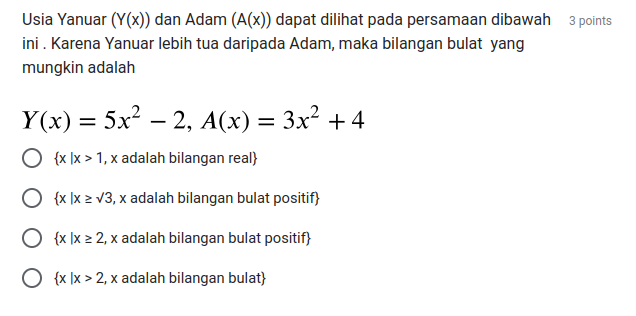
\includegraphics[width=\linewidth]{img/img09}
		\end{center}
	\end{frame}
	
	\begin{frame}
		\frametitle{Pembahasan Soal Pretest}
		\begin{center}
			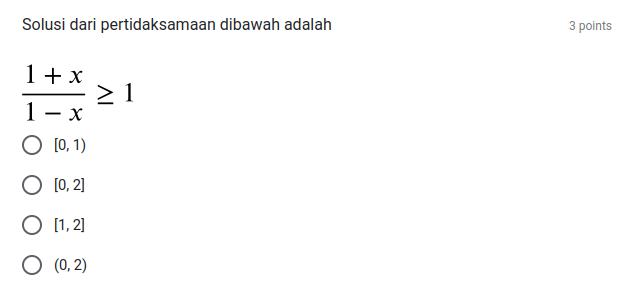
\includegraphics[width=\linewidth]{img/img10}
		\end{center}
	\end{frame}
	
	\begin{frame}
		\frametitle{Pembahasan Soal Pretest}
		\begin{center}
			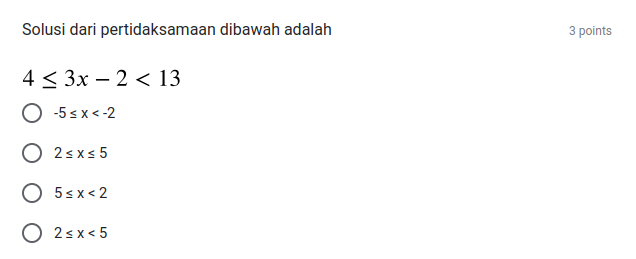
\includegraphics[width=\linewidth]{img/img11}
		\end{center}
	\end{frame}
	
	\begin{frame}
		\frametitle{Pembahasan Soal Pretest}
		\begin{center}
			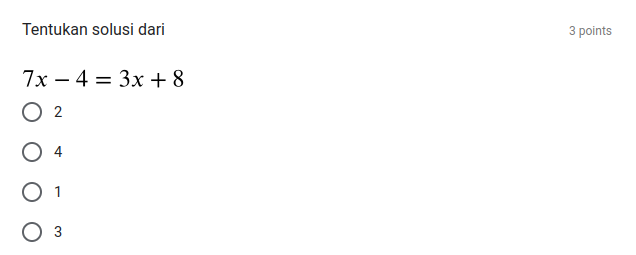
\includegraphics[width=\linewidth]{img/img12}
		\end{center}
	\end{frame}
	
	\begin{frame}
		\frametitle{Pembahasan Soal Pretest}
		\begin{center}
			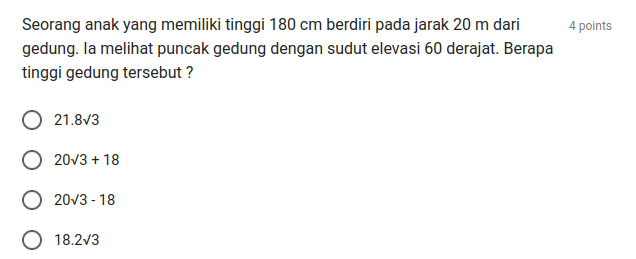
\includegraphics[width=\linewidth]{img/img13}
		\end{center}
	\end{frame}
	
	\begin{frame}
		\frametitle{Pembahasan Soal Pretest}
		\begin{center}
			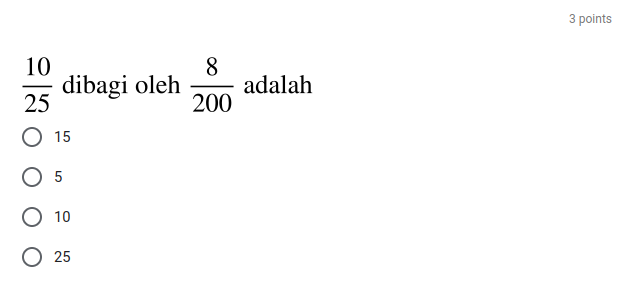
\includegraphics[width=\linewidth]{img/img14}
		\end{center}
	\end{frame}
	
	\begin{frame}
		\frametitle{Pembahasan Soal Pretest}
		\begin{center}
			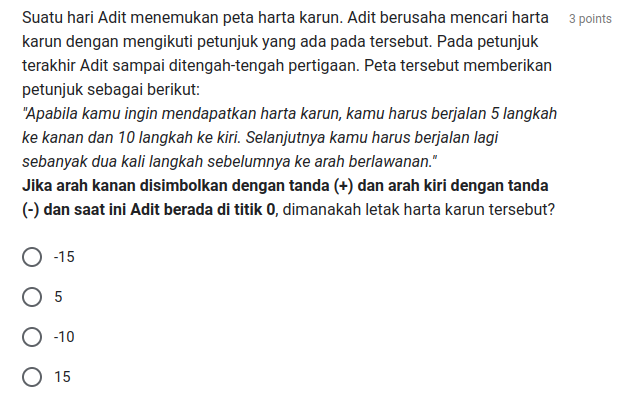
\includegraphics[width=\linewidth]{img/img15}
		\end{center}
	\end{frame}
	
	\begin{frame}
		\frametitle{Pembahasan Soal Pretest}
		\begin{center}
			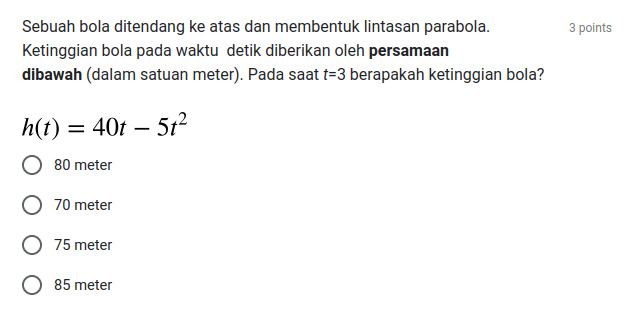
\includegraphics[width=\linewidth]{img/img16}
		\end{center}
	\end{frame}
	
	\begin{frame}
		\frametitle{Pembahasan Soal Pretest}
		\begin{center}
			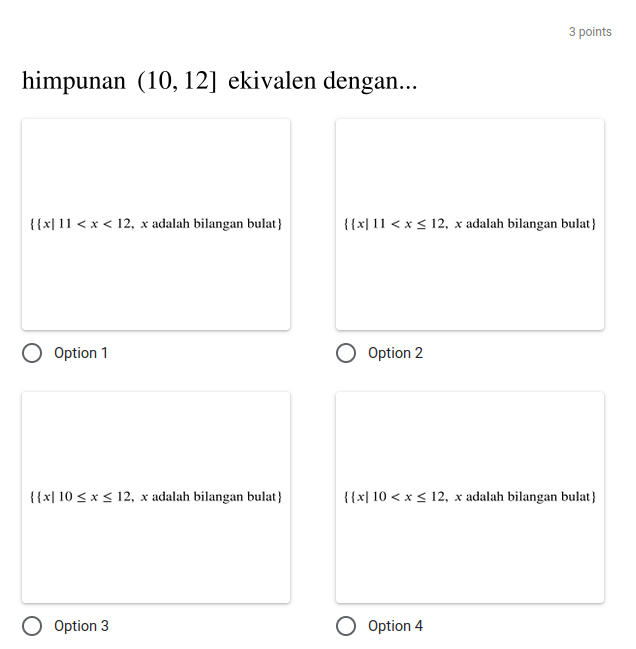
\includegraphics[width=0.6\linewidth]{img/img17}
		\end{center}
	\end{frame}
	
	\begin{frame}
		\frametitle{Pembahasan Soal Pretest}
		\begin{center}
			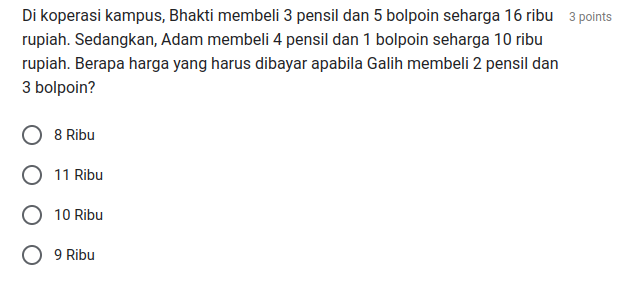
\includegraphics[width=\linewidth]{img/img18}
		\end{center}
	\end{frame}
	
	\begin{frame}
		\frametitle{Pembahasan Soal Pretest}
		\begin{center}
			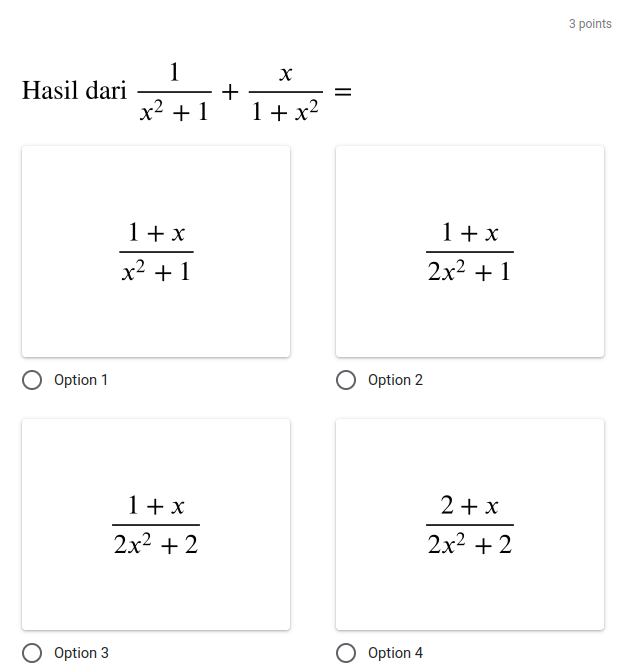
\includegraphics[width=0.6\linewidth]{img/img19}
		\end{center}
	\end{frame}
	
	\begin{frame}
		\frametitle{Pembahasan Soal Pretest}
		\begin{center}
			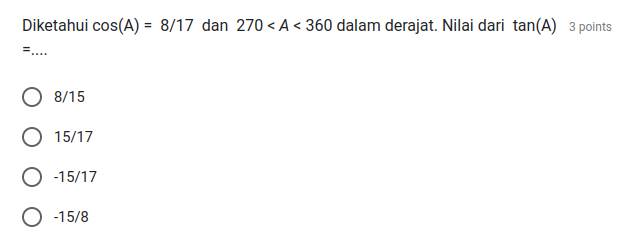
\includegraphics[width=\linewidth]{img/img20}
		\end{center}
	\end{frame}
	
	\begin{frame}
		\frametitle{Pembahasan Soal Pretest}
		\begin{center}
			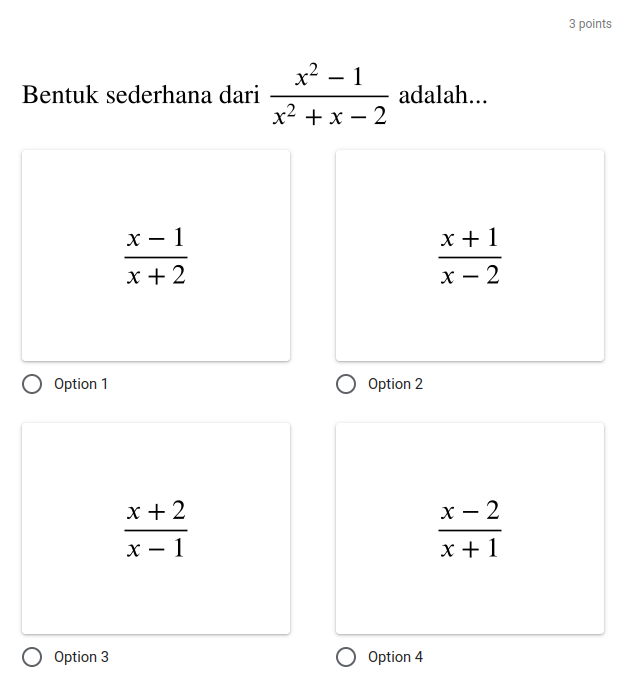
\includegraphics[width=0.6\linewidth]{img/img21}
		\end{center}
	\end{frame}
	
	\begin{frame}
		\frametitle{Pembahasan Soal Pretest}
		\begin{center}
			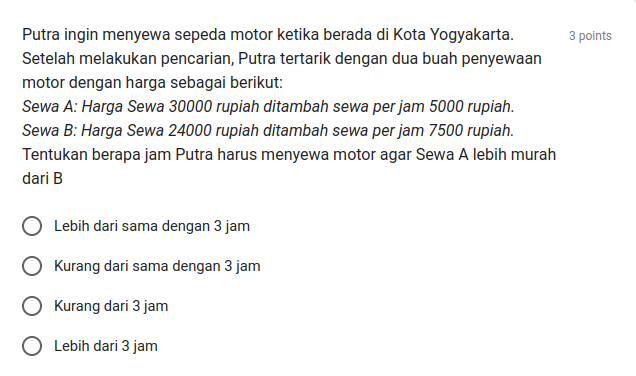
\includegraphics[width=\linewidth]{img/img22}
		\end{center}
	\end{frame}
	
	\begin{frame}
		\frametitle{Pembahasan Soal Pretest}
		\begin{center}
			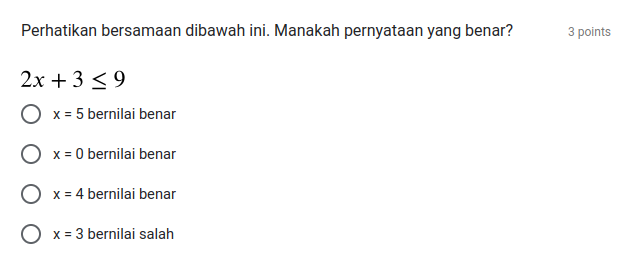
\includegraphics[width=\linewidth]{img/img23}
		\end{center}
	\end{frame}
	
	\begin{frame}
		\frametitle{Pembahasan Soal Pretest}
		\begin{center}
			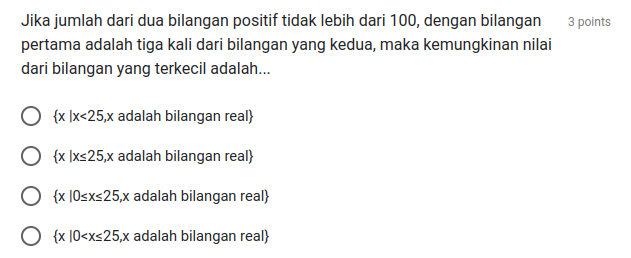
\includegraphics[width=\linewidth]{img/img24}
		\end{center}
	\end{frame}
	
	\begin{frame}
		\frametitle{Pembahasan Soal Pretest}
		\begin{center}
			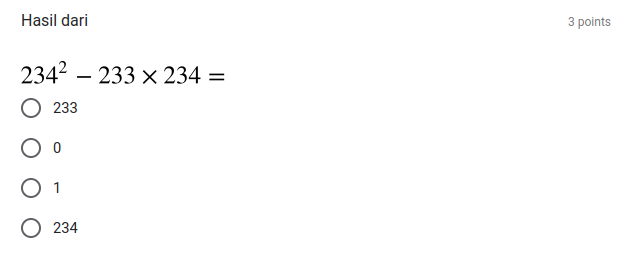
\includegraphics[width=\linewidth]{img/img25}
		\end{center}
	\end{frame}
	
	\begin{frame}
		\frametitle{Pembahasan Soal Pretest}
		\begin{center}
			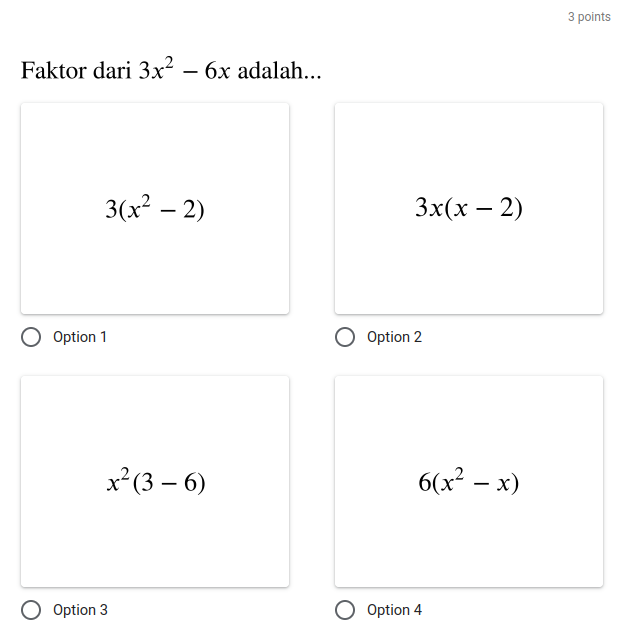
\includegraphics[width=0.6\linewidth]{img/img26}
		\end{center}
	\end{frame}
	
	\begin{frame}
		\frametitle{Pembahasan Soal Pretest}
		\begin{center}
			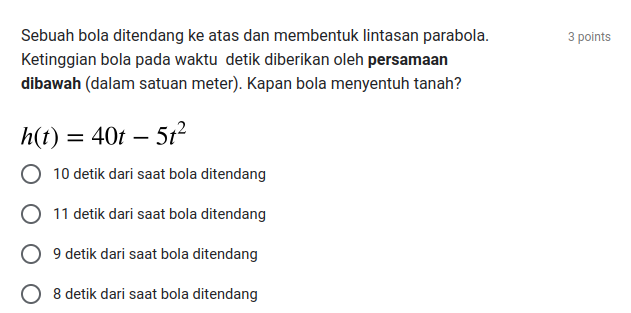
\includegraphics[width=\linewidth]{img/img27}
		\end{center}
	\end{frame}
	
	\begin{frame}
		\frametitle{Pembahasan Soal Pretest}
		\begin{center}
			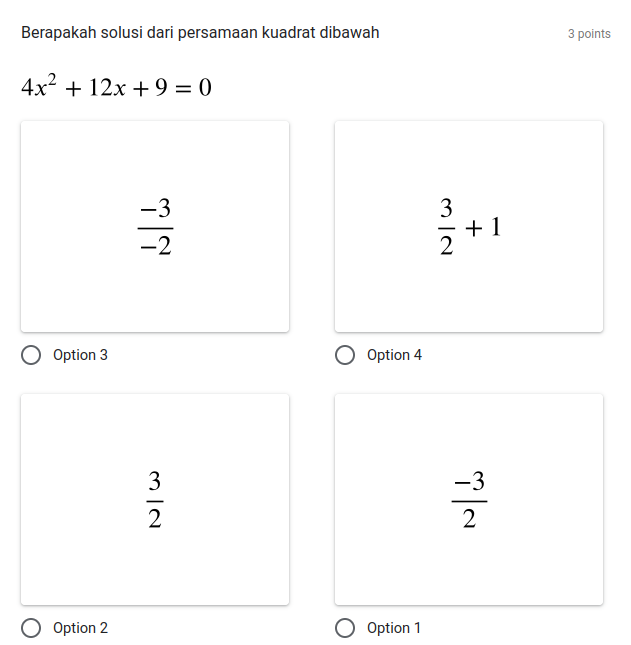
\includegraphics[width=0.6\linewidth]{img/img28}
		\end{center}
	\end{frame}
	
	\begin{frame}
		\frametitle{Pembahasan Soal Pretest}
		\begin{center}
			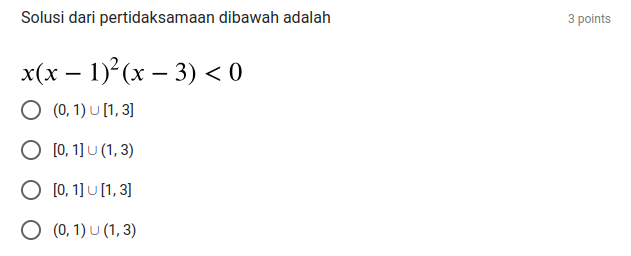
\includegraphics[width=\linewidth]{img/img29}
		\end{center}
	\end{frame}
	
	\begin{frame}
		\frametitle{Pembahasan Soal Pretest}
		\begin{center}
			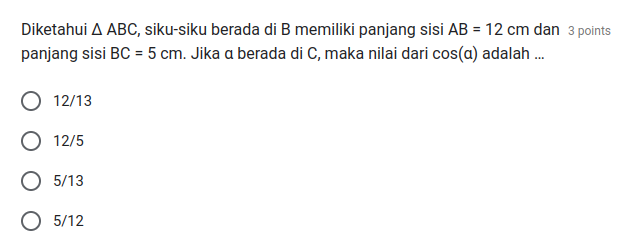
\includegraphics[width=\linewidth]{img/img30}
		\end{center}
	\end{frame}
	
	\begin{frame}
		\frametitle{Pembahasan Soal Pretest}
		\begin{center}
			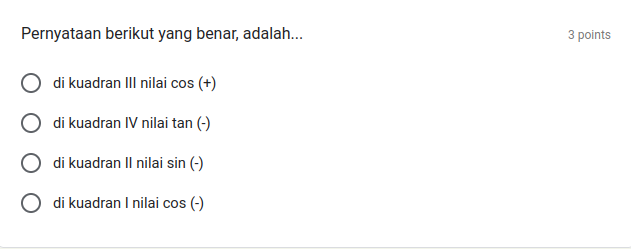
\includegraphics[width=\linewidth]{img/img31}
		\end{center}
	\end{frame}
	
	\begin{frame}
		\frametitle{Pembahasan Soal Pretest}
		\begin{center}
			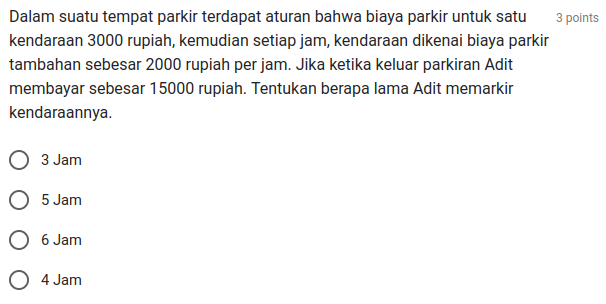
\includegraphics[width=\linewidth]{img/img32}
		\end{center}
	\end{frame}
	
	\begin{frame}
		\frametitle{Pembahasan Soal Pretest}
		\begin{center}
			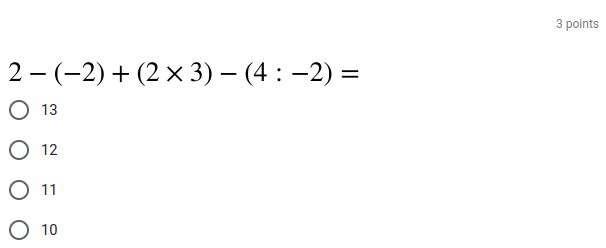
\includegraphics[width=\linewidth]{img/img33}
		\end{center}
	\end{frame}
	
	
\end{document}
